% !TeX spellcheck = pt_BR
% !TeX encoding = UTF-8
% Escolha: portugues ou ingles ou espanhol.
% Para a versão final do texto, após a defesa acrescente final:

% Para o exame de qualificação
%\documentclass[portugues, qualificacao]{ic-tese}
% Para a tese
\documentclass[portugues]{ic-tese}
% Para a versão final da tese
%\documentclass[portugues,final]{ic-tese}

% Extra macros para escrita 
%\usepackage{ic-extras}

\usepackage[latin1,utf8]{inputenc}
\usepackage{pifont}

%% Math
\usepackage{mathtools}
\usepackage{amsmath}
\usepackage{commath}

\usepackage{amsfonts}% revise se precisa ou não
\usepackage{nccmath}% revise se precisa ou não

\usepackage[numbers]{natbib}
\usepackage{multirow}
\usepackage{makecell}
\usepackage{graphicx}

\usepackage{listings}

\renewcommand{\lstlistingname}{Código}
\renewcommand{\lstlistlistingname}{Lista de \lstlistingname s}

\definecolor{codegreen}{rgb}{0,0.6,0}
\definecolor{codegray}{rgb}{0.85,0.85,0.85}
\definecolor{codepurple}{rgb}{0.58,0,0.82}
\definecolor{codeblack}{rgb}{0,0,0}

\lstdefinestyle{codigo}{
    backgroundcolor=\color{codegray},   
    commentstyle=\color{codegreen},
    keywordstyle=\color{magenta},
    numberstyle=\tiny\color{codeblack},
    stringstyle=\color{codepurple},
    basicstyle=\ttfamily\footnotesize,
    breakatwhitespace=false,         
    breaklines=true,                 
    captionpos=b,                    
    keepspaces=true,                 
    numbers=left,                    
    numbersep=5pt,                  
    showspaces=false,                
    showstringspaces=false,
    showtabs=false,                  
    tabsize=4
}

\lstset{style=codigo}

\newcommand\citetxt[1]{%
  \citeauthor{#1}~(\citeyear{#1})}
\newcommand\citepar[1]{%
  (\citeauthor{#1}, \citeyear{#1})} 


%% tight space around equations
%\apptocmd\normalsize{%
%  \abovedisplayskip=7pt plus 2pt minus 7pt
%  \abovedisplayshortskip=0pt plus 3pt
%  \belowdisplayskip=7pt plus 2pt minus 6pt
%  \belowdisplayshortskip=4pt plus 3pt minus 4pt
%}{}{}
%
%\abovedisplayskip=0pt
%\belowdisplayskip=0pt

\newcommand{\conc}{\mathbin{\Vert}}

% Adaptive norm operator
% https://tex.stackexchange.com/a/70130/7561
% With this setup, \norm*{...} will produce automatically sized double-bar
% fence symbols around the macro's, whereas (say) \norm[\bigg]{...} will
% generate \bigg double-bar symbols. There are four sizing modifiers: \big,
% \Big, \bigg, and \Bigg. 

%https://tex.stackexchange.com/q/151984/7561
\DeclarePairedDelimiterX{\infdivx}[2]{(}{)}{%
  #1\;\delimsize\|\;#2%
}
\newcommand{\kl}{\operatorname{KL}\infdivx}
\newcommand{\skl}{\operatorname{SKL}\infdivx}

% https://tex.stackexchange.com/questions/23773/a-centered-plus-minus-symbol
\newcommand{\rpm}{\raisebox{.2ex}{$\scriptstyle\pm$}}

% https://tex.stackexchange.com/a/141685/7561
\newcommand\givenbase[1][]{\:#1\lvert\:}
\let\given\givenbase

% https://tex.stackexchange.com/a/171959/7561
\newcommand\reallywidehat[1]{\ThisStyle{%
    \setbox0=\hbox{$\SavedStyle#1$}%
    \stackengine{-1.0\ht0+.5pt}{$\SavedStyle#1$}{%
      \stretchto{\scaleto{\SavedStyle\mkern.15mu\char'136}{1.5\wd0}}{1.4\ht0}%
    }{O}{c}{F}{T}{S}%
}}
\newcommand{\hkl}{\widehat{\operatorname{KL}}\infdivx}

% Conditional independence symbol
% https://tex.stackexchange.com/questions/218631/symbol-for-not-conditionally-independent/
\newcommand{\CI}{\mathrel{\perp\mspace{-10mu}\perp}}

% declare my argmin and argmax operators
% https://tex.stackexchange.com/a/5255/7561
\DeclareMathOperator*{\argmax}{arg\,max}
\DeclareMathOperator*{\argmin}{arg\,min}

% declaring an expectation operator to behave like sum
% https://tex.stackexchange.com/a/23436/7561
\makeatletter
\DeclareRobustCommand\bigop[1]{%
  \mathop{\vphantom{\sum}\mathpalette\bigop@{#1}}\slimits@
}
\newcommand{\bigop@}[2]{%
  \vcenter{%
    \sbox\z@{$#1\sum$}%
    \hbox{\resizebox{\ifx#1\displaystyle.9\fi\dimexpr\ht\z@+\dp\z@}{!}{$\m@th#2$}}%
  }%
}
\makeatother

%\newcommand{\E}{\DOTSB\bigop{\mathbb{E}}}
\DeclareMathOperator*{\E}{\mathbb{E}}

% redefining \times operator
\let\oldtimes\times
\def\times{{\mkern1mu\oldtimes\mkern1mu}}



\usepackage{subfigure}
\newcommand{\cmark}{\ding{51}}%

%\DeclarePairedDelimiter\abs{\lvert}{\rvert}%
%\DeclarePairedDelimiter\norm{\lVert}{\rVert}%
\DeclarePairedDelimiter\product{\langle}{\rangle}%

\usepackage{cellspace}
\setlength\cellspacetoplimit{6pt}
\setlength\cellspacebottomlimit{4pt}

%% Units
\usepackage{siunitx}

%% Tables
\usepackage{booktabs}


% Para acrescentar comentários ao PDF descomente:
\usepackage
%  [pdfauthor={nome do autor},
%   pdftitle={titulo},
%   pdfkeywords={palavra-chave, palavra-chave},
%   pdfproducer={Latex with hyperref},
%   pdfcreator={pdflatex}]
{hyperref}

% Os cores podem ser mudados
\hypersetup{
%  linkcolor={red!50!black},
%  citecolor={blue!50!black},
%  urlcolor={blue!80!black}
}

\begin{document}

% Escolha entre autor ou autora:
\autor{Thales Eduardo Nazatto}
%\autora{Nome da Autora}

% Sempre deve haver um título em português:
\titulo{Construção de um \textit{Pipeline} de \textit{Machine Learning} autônomo com métricas de \textit{Fairness}}
\title{text}

% Se a língua for o inglês ou o espanhol defina:
%\title{The Dissertation or Thesis Title in English or Spanish}

% Escolha entre orientador ou orientadora. Inclua os títulos acadêmicos:
%\orientador{Prof. Dr. Gerberth Adín Ramírez Rivera}
\orientadora{Profa. Dra. Cecília Mary Fischer Rubira}

% Escolha entre coorientador ou coorientadora, se houver.  Inclua os títulos acadêmicos:
\coorientador{Prof. Dr. Leonardo Montecchi}
%\coorientadora{Prof. Dra. Eng. Lic. Nome da Co-Orientadora}

% Escolha entre mestrado ou doutorado:
\mestrado
%\doutorado

% Se houve cotutela, defina:
%\cotutela{Universidade Nova de Plutão}

\datadadefesa{30}{07}{2022}

% Para a versão final defina:
%\avaliadorA{Prof. Dr. Primeiro Avaliador}{Instituição do primeiro avaliador}
%\avaliadorB{Profa. Dra. Segunda Avaliadora}{Instituição da segunda avaliadora}
%\avaliadorC{Dr. Terceiro Avaliador}{Instituição do terceiro avaliador}
%\avaliadorD{Prof. Dr. Quarto Avaliador}{Instituição do quarto avaliador}
%\avaliadorE{Prof. Dr. Quinto Avaliador}{Instituição do quinto avaliador}
%\avaliadorF{Prof. Dr. Sexto Avaliador}{Instituição do sexto avaliador}
%\avaliadorG{Prof. Dr. Sétimo Avaliador}{Instituição do sétimo avaliador}
%\avaliadorH{Prof. Dr. Oitavo Avaliador}{Instituição do oitavo avaliador}


% Para incluir a ficha catalográfica em PDF na versão final, descomente e ajuste:
%\fichacatalografica{arquivo.pdf}


% Este comando deve ficar aqui:
\frontmatter


% Se houver dedicatória, descomente:
%\prefacesection{Dedicatória}
%A dedicatória deve ocupar uma única página.

% Se houver epígrafe, descomente e edite:
\begin{epigrafe}
{\it
Alguma frase\\
Para colocar,\\
Mas é um dos últimos itens a se fazer.}

\hfill (Eu mesmo)
\end{epigrafe}


% Agradecimentos ou Acknowledgements ou Agradecimientos
\chapter{Agradecimentos}
%Os agradecimentos devem ocupar uma única página.
Agradecer posteriormente


% Sempre deve haver um resumo em português:
\begin{resumo}
Esta dissertação de Mestrado possui o objetivo de contribuir com o tema de Inteligência Artificial (IA) do ponto de vista da Engenharia de Software, visto que o uso de IA envolvendo grandes volumes de dados vem crescendo conforme nossa sociedade migra processos manuais de trabalho para soluções digitais e necessita de tomadas de decisão mais rápidas e assertivas. Entretanto, as métricas usadas inicialmente para definir a eficácia de um algoritmo se mostraram limitadas devido a barreiras éticas e legais, resultando em vieses que refletem a sociedade de maneira que não era esperada pelos desenvolvedores da solução. Desta forma, o uso de novas métricas, como métricas de Fairness, e proveniência de dados pode ajudar neste problema. Desenvolvendo um pipeline autônomo utilizando a arquitetura MAPE-K, documentando métodos e ferramentas, e realizando estudos de caso, é esperado que este problema seja controlado e facilite o desenvolvimento de softwares com o uso responsável de dados.
\end{resumo}


% Sempre deve haver um abstract:
\begin{abstract}
This Master's Degree dissertation aims to contribute to the theme of Artificial Intelligence (AI) from the Software Engineering point of view, since the use of AI involving large volumes of data has been growing as our society migrates manual work processes to digital solutions and needs faster and more assertive decision making. However, the metrics used initially to define the effectiveness of an algorithm proved to be limited due to ethical and legal barriers, resulting in biases that reflect society in a way that was not expected by the solution developers. Thus, the use of new metrics, like Fairness metrics, and data provenance can help with this problem. By developing an autonomous pipeline using MAPE-K architecture, documenting methods and tools, and making case studies, it is expected that this problem will be controlled and facilitate software development with the responsible use of data.
\end{abstract}


% Se houver um resumo em espanhol, descomente:
%\begin{resumen}
% A mesma regra aplica-se.
%\end{resumen}


% A lista de figuras é opcional:
\listoffigures

% A lista de tabelas é opcional:
% \listoftables

% A lista de abreviações e siglas é opcional:
% \prefacesection{Lista de Abreviações e Siglas}

% A lista de símbolos é opcional:
% \prefacesection{Lista de Símbolos}

% Quem usa o pacote nomencl pode incluir:
%\renewcommand{\nomname}{Lista de Abreviações e Siglas}
%\printnomenclature[3cm]


% O sumário vem aqui:
\tableofcontents


% E esta linha deve ficar bem aqui:
\mainmatter

%\mainmatter

\chapter{Introdução}

% O corpo da dissertação ou tese começa aqui:
Técnicas de Inteligência Artificial e Aprendizado de Máquina já são utilizadas há bastante tempo no ramo da Computação. Ramos como robótica e jogos são grandes exemplos, dada a necessidade nos mesmos de automatizar comportamentos que seriam tidos como triviais para um ser humano. Entretanto, nos últimos anos ocorreu um crescimento no uso dessas tecnologias em aplicações tradicionais, com previsão de US\$ 57 bilhões em investimentos em 2021, 480\% maior em relação a 2017~\citep{Deloitte_2018}. No Brasil, o número de empresas de IA aumentou de 120 em 2018 para 206 em 2020~\citep{CIO_2021}.

Isso se mostra possível devido a grande quantidade de dados processada diariamente pelas empresas, que coletam estatísticas toda vez que um usuário acessa suas aplicações. Com esses dados, podem traçar diferentes perfis e usar soluções de IA para ter tomadas de decisão mais assertivas com o objetivo de melhorar a experiência de usuário e corrigir problemas. Porém, muitas dessas soluções foram projetadas sem pensar em governança de dados como requisito de projeto, e se mostram ineficientes quando ela é tratada em consideração.

Governança de dados é um tema que entrou em evidência recentemente em países como o Brasil: Iniciativas como a LGPD - Lei Geral de Proteção de Dados \citep{LGPD_2021}, de 14 de agosto de 2018, mostram como as aplicações e seus dados possuem cada vez mais influência na sociedade moderna. E nesse ponto muitas aplicações de IA falham: muitas implementações foram implementadas como \textit{black boxes}, onde o determinante para estabelecer a confiança no modelo implementado é sua entrada e sua saída.

Um outro efeito colateral dessa estratégia é a exposição de vieses que, embora sejam vistos como não-intencionais pelos desenvolvedores por ter a possibilidade de ser um \textit{outlier} no modelo treinado, refletem preconceitos escancarados da sociedade atual. Uma entrada de dados enviesada resulta em um algoritmo que realiza discriminações em sua classificação~\citep{Buolamwini_2018}, e uma vez que as métricas utilizadas para medir a qualidade de um modelo \textit{black box} são geralmente baseadas em acurácia, precisão e recall, discriminações não são facilmente percebidas por tais métricas. Ao mesmo tempo, um modelo \textit{black box} pode ter uma alta dependência de poucos dados, determinando problemas de acoplamento. Para resolver este problema, é possível que a criação de um novo modelo seja uma melhor opção que realizar a correção em apenas parte dele.

Devido a esses tipos de problemas, o termo \textit{Explainable AI} (XAI) ganha força para envolver o desenvolvimento de uma IA que seja acurada e simultaneamente transparente. Como IA possui diversos tipos de métodos diferentes para enquadrar diversos tipos de dados, o mesmo acaba se aplicando em Explainable AI, podendo enquadrar em diversos tipos de dados~\citep{Sundararajan_2017}, ou dados específicos como imagens~\citep{Kapishnikov_2019} e tabelas~\citep{Maleki_2013}. Como o objetivo em XAI é fazer com que os resultados alcançados pela solução de IA sejam compreendidos por humanos, é possível considerar este fato como requisito no design de uma solução de IA, fazendo com que a mesma seja reusável e testável.

No mesmo tema, é possível estabelecer métricas para determinar o quão o modelo está preparado para dados sensíveis \citep{Begley_2021}, termo que é conhecido como \textit{Fairness}. Com a evolução das pesquisas na comunidade acadêmica, foram descobertos algoritmos para redução dos vieses presentes nos conjuntos de dados, como \textit{Reweighing}~\citep{Kamiran_2011}, \textit{Adversarial Debiasing}~\citep{Zhang_2018} e \textit{Reject Option Classification}~\citep{Kamiran_2012}. Por consequência, ocorre melhora nas métricas em questão, mas pode desfavorecer métricas que já são amplamente utilizadas como garantia de um bom modelo desenvolvido com técnicas de Aprendizado de Máquina.

O objetivo desta dissertação de mestrado é desenvolver uma estrutura de \textit{Pipeline} para \textit{Machine Learning} que seja completamente autônoma, por três fatores principais:

\begin{itemize}
\item Facilitar a criação de modelos justos e confiáveis com a automatização da escolha dos algoritmos, cuja complexidade aumenta com a escolha dos algoritmos a serem utilizados e suas execuções nas etapas corretas do processo, onde eles foram escolhidos para atuar.
\item Estabelecer um balanceamento entre métricas para avaliar bons modelos com métricas para avaliar modelos justos.
\item Considerar proveniência de dados como requisito no design de uma solução de IA, e como uma alternativa a XAI através da utilização de metadados.
\end{itemize}

Para isso, além do desenvolvimento do \textit{Pipeline} em questão, será utilizada a arquitetura MAPE-K~\citep{IBM_2005} para analisar uma base de conhecimento e prover o melhor pipeline seguindo regras pré-determinadas.

O restante da dissertação se organizará da seguinte forma: o Capítulo 2 descreve os conceitos que irão ser abordados neste projeto; o Capítulo 3 mostra a metodologia e detalhamento do processo de desenvolvimento; o Capítulo 4 discute os resultados obtidos e, finalmente, o Capítulo 5 estabelece as conclusões, considerações finais e sugestões de trabalhos futuros e evoluções.

\chapter{Conceitos Relacionados}

\section{Ciência de Dados e Engenharia de Dados}

\section{Machine Learning}

Aprendizado de Máquina (\textit{Machine Learning}, em inglês) pode ser definido como “a prática de usar algoritmos para coletar dados, aprender com eles, e então fazer uma determinação ou predição sobre alguma coisa no mundo. Então em vez de implementar as rotinas de software manualmente, com um gama específica de instruções para completar uma tarefa em particular, a máquina é `treinada` usando uma quantidade grande de dados e algoritmos que dão e ela a habilidade de aprender como executar a tarefa”~\citep{Copeland_2016}. Com isso, o computador consegue a habilidade de realizar determinado cálculo ou tarefa sem que necessite de programação adicional ou interferência humana para isso.

O \textit{Machine Learning} é fortemente relacionado com a Estatística, uma vez que seus métodos e parte de seus algoritmos, como regressões, tiveram como base modelos estatísticos e a análise de seus dados. As tarefas de aprendizado podem ser classificadas em três categorias básicas~\citep{MLWikipedia_2021}~\citep{MLSAS_2021}:

\begin{itemize}
\item \textbf{Aprendizado supervisionado}: O treinamento é realizado por meio de exemplos rotulados, como uma entrada na qual a saída desejada é conhecida. Através de métodos como classificação, regressão e \textit{gradient boosting}, o aprendizado supervisionado utiliza padrões para prever os valores de rótulos em dados não-rotulados adicionais. O aprendizado supervisionado é comumente empregado em aplicações nas quais dados históricos preveem eventos futuros prováveis.
\item \textbf{Aprendizado não-supervisionado}: É utilizado em dados que não possuem rótulos históricos. A “resposta certa” não é informada ao sistema, o algoritmo deve descobrir o que está sendo mostrado. O objetivo é explorar os dados e encontrar alguma estrutura dentro deles. Técnicas populares incluem mapas auto-organizáveis, mapeamento por proximidade, agrupamento \textit{k-means} e decomposição em valores singulares. Esses algoritmos também são utilizados para segmentar tópicos de texto, recomendar itens e identificar pontos discrepantes nos dados.
\item \textbf{Aprendizado por reforço}: O algoritmo descobre através de testes do tipo “tentativa e erro” quais ações rendem as maiores recompensas. Este tipo de aprendizado possui três componentes principais: o agente (o aprendiz ou tomador de decisão), o ambiente (tudo com que o agente interage) e ações (o que o agente pode fazer). O objetivo é que o agente escolha ações que maximizem a recompensa esperada em um período de tempo determinado. O agente atingirá o objetivo muito mais rápido se seguir uma boa política, então o foco do aprendizado por reforço é descobrir a melhor política.
\end{itemize}

O termo \textit{Machine Learning} se tornou muito mais evidente com a possibilidade da implementação do \textit{Deep Learning}, que é uma técnica que utiliza Redes Neurais Artificiais para atingir seus resultados. Redes Neurais Artificiais são modelos computacionais inspirados no sistema nervoso do cérebro, onde temos neurônios divididos em camadas e conectados entre si, podendo ser abstraído conforme ilustração na Figura \ref{fig:NeuralNetwork}. Dependendo da tarefa a ser realizada, cada neurônio atribui um peso para os dados que entram e a saída final é determinada pelo total desses pesos~\citep{Copeland_2016}. As redes neurais utilizadas em \textit{Deep Learning} possuem, ao menos, duas camadas de neurônios entre a camada que recebe os dados de entrada e a camada final que faz o tratamento final dos dados de saída.

\begin{figure}[h]
\centering
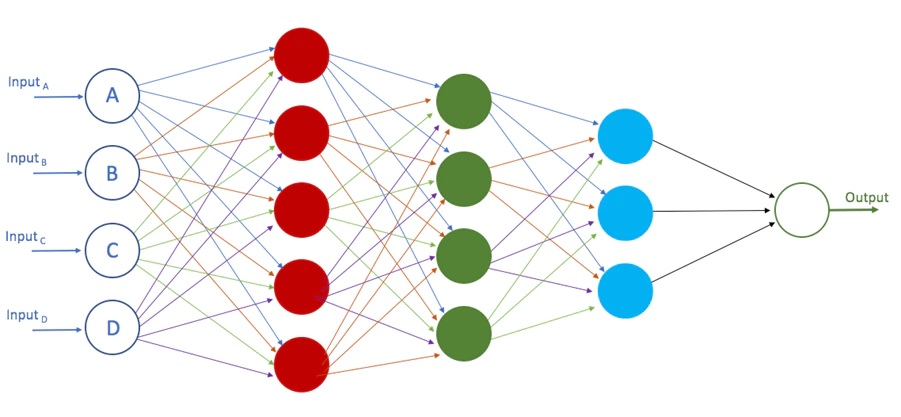
\includegraphics[scale=0.8]{images/deep_neural_network.jpg}
\caption {Exemplo de uma rede neural utilizada em \textit{Deep Learning}.}
\label{fig:NeuralNetwork}
\end{figure}

Com a evolução da computação, o treino de uma tarefa passou a ser cada vez mais viável, uma vez que a execução de algoritmos de \textit{Machine Learning} é computacionalmente muito custosa, especialmente quando redes neurais são utilizadas. E sua viabilidade é acompanhada de efetividade: Como exemplo, reconhecimento de imagens por máquinas treinadas através de deep learning em alguns cenários possuem uma taxa de acerto maior que a de humanos~\citep{Copeland_2016}.

\subsection{Métricas de Avaliação}

Tradicionalmente em um problema de classificação binária, uma previsão do classificador pode ter 4 tipos de resultados em uma matriz de confusão, presente na Tabela \ref{tbl:ConfusionMatrix}. Os Verdadeiros Positivos (VP, ou TP pelo termo em inglês \textit{True Positives}) e Verdadeiros Negativos (VN, ou TN pelo termo em inglês \textit{True Negatives}) são classificações corretamente previstas pelo classificador. Um Falso Positivo (FP) ocorre quando um caso previsto para estar na classe positiva quando o resultado real pertence à classe negativa, e um Falso Negativo (FN) ocorre quando um caso previsto para estar na classe negativa
quando o resultado real pertence à classe positiva.

-- TODO reformatar Tabela

\begin{table}[h]
\label{tbl:ConfusionMatrix}
\begin{center}
  \caption{Matriz de confusão}
  \resizebox{\linewidth}{!}{%
  \begin{tabular}{|c|c|c|c|}
    \toprule
    \multicolumn{4}{|c|}{Classe prevista}\\
    \midrule
    \multirow{3}{*}[-3ex]{\rotatebox[origin=c]{90}{\textbf{Classe atual}}} &  & \textbf{Positiva} & \textbf{Negativa}\\[3ex]
    \cmidrule{2-4}
     & \textbf{Positiva} & \makecell{Verdadeiros Positivos\\(VP/TP)} & \makecell{Falsos Positivos\\(FP)}\\[3ex]
    \cmidrule{2-4}
     & \textbf{Negativa} & \makecell{Falso Negativo\\(FN)} & \makecell{Verdadeiros Negativos\\(VN/TN)}\\[3ex]
    \bottomrule
  \end{tabular}}
\end{center}
\end{table}

A taxa de sucesso, também conhecida como \textbf{acurácia}, é o número de previsões corretas dividido pelo número total de resultados:

\begin{equation}
Acc = \frac{TP + TN}{TP + TN + FP + FN}
\end{equation}

Ela é considerada um indicador da realização de um bom treinamento e de um bom funcionamento do modelo obtido. Entretanto, não é a melhor métrica para interpretar situações quanto a aplicação do modelo ao problema, como classes desequilibradas.

A \textbf{precisão} ajuda quando os custos de falsos positivos são altos e mostra a precisão das previsões positivas. É a fração de casos positivos previstos corretamente para estar na classe positiva de todos os casos positivos previstos no modelo:

\begin{equation}
P = \frac{TP}{TP + FP}
\end{equation}

O \textbf{recall}, ou sensibilidade, ajuda quando o custo de falsos negativos é alto.  É a fração de casos positivos previstos corretamente para estar na classe positiva de todos os casos positivos reais:

\begin{equation}
R = \frac{TP}{TP + FN}
\end{equation}

O \textbf{F1-score} é uma medida geral da acurácia de um modelo que combina precisão e recall. Pode ser interpretado como uma ponderação entre ambos e usa a média harmônica para realizar a medição:

\begin{equation}
F1 = 2 \times\frac{P \times R}{P + R}
\end{equation}

O \textbf{AUC} (\textit{Area under the ROC Curve}), também chamada de precisão balanceada, pode imterpretar a capacidade do classificador de evitar uma classificação falsa. Se sai melhor que a acurácia em situações que ela não é apropriada, como o desequilíbrio entre classes já citado anteriormente:

\begin{equation}
AUC = \frac{1}{2} \left( \frac{TP}{TP + FN} + \frac{TN}{TN + FP} \right)
\end{equation}

\subsection{Algoritmos}

\section{Fairness em Machine Learning}

Como a coleta de dados está presente atualmente no dia-a-dia de variados setores da sociedade, o uso de \textit{Machine Learning} é extremamente versátil para tomadas de decisão, podendo ser utilizados em problemas como admissão de universidades, contratações, análise de crédito e reconhecimento de doenças. Com o aumento dessa influência, o uso de dados sensíveis em um contexto determinado também aumentou, e temas como uma IA ética e conceitos como vieses nos dados e \textit{Fairness} passaram a serem discutidas não apenas na Computação, mas em áreas como Direito. Algoritmos são mais objetivos, rápidos e são capazes de considerar uma grande magnitude de recursos que pessoas não são capazes. Entretanto, até o presente momento eles não são capazes de diferenciar contextos sociais, onde um resultado mais eficiente de acordo com os dados disponíveis podem amplificar as desigualdades sociais e tomar decisões de modo injusto~\citep{Mehrabi_2021}. 

Estes dados sensíveis, tendo como exemplos cor de pele, raça, sexo, idade e altura, são considerados atributos protegidos, que precisam ser classificados e processados antes da execução de um algoritmo de \textit{Machine Learning}, determinarão como o algoritmo se comportará e, consequentemente, afetará suas métricas~\citep{Mougan_2022}. Os grupos de dados provenientes destes atributos protegidos são considerados grupos protegidos, que podem ser divididos em dois grupos: o grupo privilegiado, que possui vantagens no contexto do problema, e o grupo não-privilegiado, que possui desvantagens no contexto do problema e, portanto, sujeito a discriminação.

É possível descrever o conceito de \textit{Fairness} no contexto de aprendizagem supervisionada, onde um modelo $f$ pode prever um conjunto de resultados $y$ a partir de um conjunto de \textit{features} $x$, evitando discriminação injusta em relação a um atributo protegido $a$. É permitido, mas não exigido, que $a$ seja um componente de $x$~\citep{Begley_2021}. Em outras palavras, um modelo de ML considerado justo é aquele onde a correlação de seu resultado é baixa em relação a dados de entrada considerados como sensíveis a discriminações.

Geralmente, as descrições de justiça se dividem em dois grupos principais: justiça individual e justiça de grupo. O objetivo da justiça individual é que indivíduos semelhantes devem obter resultados semelhantes, enquanto na justiça de grupo, cada um dos grupos definidos pelo atributo protegido deve ser tratado igualmente.
ser tratados igualmente.

-- TODO continuar

\subsection{Métricas de Fairness}

Considerando $Y=1$ a classe positiva, $Z=0$ o grupo não-privilegiado e $Z=1$ o grupo privilegiado, algumas das definições de \textit{Fairness} mais usadas são as seguintes:

\begin{itemize}
\item \textbf{Diferença de paridade estatística, ou discriminação~\citep{Zemel_2013}:} Esta métrica é baseada na seguinte fórmula:

\begin{equation}
Pr(Y=1|Z=0)-Pr(Y=1|Z=1)
\end{equation}
 
Aqui, o viés ou paridade estatística é a diferença entre a probabilidade de que um indivíduo aleatório retirado dos não-privilegiados seja rotulado como 1 e a probabilidade de que um indivíduo aleatório dos privilegiados seja rotulado como 1. Portanto, um valor próximo de 0 é considerado justo.

\item \textbf{Diferença de oportunidade igual~\citep{Biswas_2020}:} É a diferença entre a taxa positiva verdadeira do grupo não privilegiado e a taxa positiva verdadeira do grupo privilegiado:

\begin{equation}
TPR_{Z=0} - TPR_{Z=1}
\end{equation}
 
Um valor próximo de 0 é considerado justo. Um classificador binário satisfaz a igualdade de oportunidades quando a taxa positiva verdadeira de ambos os grupos são iguais~\citep{Hardt_2016}

\item \textbf{Diferença de probabilidade média~\citep{Biswas_2020}:} Essa métrica usa a taxa de falsos positivos e a taxa positiva verdadeira para calcular a tendência, calculando a igualdade de probabilidades com a fórmula:

\begin{equation}
\frac{1}{2}(|FPR_{Z=0} - FPR_{Z=1}|+|TPR_{Z=0} - TPR_{Z=1}|)
\end{equation}
 
Precisa ser próximo a 0 para ser considerado justo.

\item \textbf{Impacto de disparidade~\citep{Biswas_2020}:} Para esta métrica, é usada a seguinte fórmula:

\begin{align*}
\frac{Pr(Y=1|Z=0)}{Pr(Y=1|Z=1)}
\end{align*}

Usa as mesmas probabilidades da diferença de paridade estatística, mas aqui são calculadas como proporção. Desta forma, um valor próximo de 1 é considerado justo.

\item \textbf{Indíce de Theil~\citep{Speicher_2018}:} Esta medida também é conhecida como índice de entropia generalizado, mas com $\alpha$ igual a 1~\citep{Speicher_2018}. É calculado com a seguinte fórmula:

\begin{align*}
\frac{1}{n}\sum^{n}_{i=0}\frac{b_i}{\mu}\ln{\frac{b_i}{\mu}}
\end{align*}

Onde $b_i = \hat{y}_i - y_i + 1$, $y_i$ é o conjunto de saídas e $\hat{y}_i$ é o conjunto de previsões dadas pelo modelo. Também precisa ser próximo a 0 para ser considerado justo.

\end{itemize}

\subsection{Algoritmos para redução de vieses}

Há diversos tipos de algoritmos diferentes na inteligência artificial para redução de vieses, a fim de garantir \textit{Fairness} nos projetos de Aprendizado de Máquina. É possível classificá-los em três categorias diferentes: Algoritmos de pré-processamento, processamento e de pós-processamento.

Os algoritmos de \textbf{pré-processamento} tentam eliminar a discriminação transformando os dados, antes de executar o algoritmo de treinamento. Tais algoritmos podem ser usados caso seja permitida a modificação dos dados de treinamento~\citep{dAlessandro_2017}, e a ideia por trás de tais algoritmos é que suas previsões serão mais balanceadas se o classificador for treinado com os dados já balanceados~\citep{Kamiran_2009}. Nesta categoria se enquadram os seguintes algoritmos:

\begin{itemize}
\item \textbf{Reposição (\textit{Reweighing})~\citep{Kamiran_2011}:} Pondera os exemplos em cada combinação de grupo e rótulo de maneira diferente para garantir a justiça antes da classificação.

\item \textbf{Removedor de impacto de disparidade (\textit{Disparate impact remover})~\citep{Feldman_2015}:} Edita valores de \textit{features} aumentando a justiça de cada grupo enquanto preserva a ordem de classificação dentro dos mesmos.

\item \textbf{Aprendizado de representações justas (LFR, ou \textit{Learning fair representations})~\citep{Zemel_2013}:} Encontra uma representação latente que codifica os dados, mas ofusca informações dos atributos protegidos.

\item \textbf{Pré-processamento otimizado (\textit{Optimized pre-processing})~\citep{Calmon_2017}:} Aprende uma transformação probabilística que edita \textit{features} e rótulos nos dados efetuando justiça em cada grupo, distorção individual, garantindo a fidelidade de dados através de restrições.
\end{itemize}

Os algoritmos de \textbf{processamento} tentam realizar modificações nos algoritmos de treinamento para mitigar a discriminação durante o processo de treinamento do modelo. Se for permitido fazer mudanças no processo de treinamento, então os algoritmos podem ser usados incorporando mudanças na função de custo ou impondo restrições~\citep{Mehrabi_2019}. Nesta categoria se enquadram os seguintes algoritmos:

\begin{itemize}
\item \textbf{Remoção de viés adversário (Adversarial debiasing)~\citep{Zhang_2018}:} Aprende um classificador que maximiza a precisão e reduz a capacidade de um adversário de depender do atributo protegido nas previsões. Essa abordagem leva a um classificador justo, pois as previsões realizadas pelo classificador não possuem nenhuma informação de discriminação nos grupos.

\item \textbf{Removedor de preconceito (Prejudice remover)~\citep{Feldman_2015}:} Técnica que adiciona no algoritmo escolhido um termo de regularização baseado na discriminação (No caso da biblioteca AI Fairness 360 é usado o programa da publicação, que usa a regressão logística como algoritmo base).

\item \textbf{Meta-Algoritmo para classificações justas (Meta-Algorithm for Fair Classification)~\citep{Celis_2019}:} Aprende um classificador compatível com uma gama grande de métricas de Fairness, sendo prático o suficiente para abrangê-las sem grande perda de performance.

\item \textbf{Justiça por Subgrupos Ricos (Rich Subgroup Fairness)~\citep{Kearns_2018}:} Aprende um classificador que procura equalizar as taxas de falsos positivos e falsos negativos entre os dados que envolvem atributos protegidos, considerados como subgrupos.

\item \textbf{Redução por Gradiente Exponencial (Exponentiated Gradient Reduction)~\citep{Agarwal_2018}:} Aprende um classificador baseado em Gradiente Exponencial que tende a minimizar o erro de uma classificação ponderada.

\item \textbf{Redução por busca em grid (Grid Search Reduction)~\citep{Agarwal_2018}~\citep{Agarwal_2019}:} Aprende um classificador baseado na busca em um grid de valores que tende a minimizar o erro de uma classificação ponderada. É mais simples e impreciso que a Redução por Gradiente Exponencial, mas sua escolha pode ser razoável se a quantidade de métricas de Fairness a serem consideradas for pequena.

\end{itemize}

Os algoritmos de \textbf{pós-processamento} utilizam um conjunto de validação, que não foi envolvido no processo de treinamento para melhorar a imparcialidade das previsões~\citep{dAlessandro_2017}. Quando não há possibilidade de fazer alterações nos dados de treinamento ou no treinamento do modelo, apenas algoritmos de pós-processamento podem ser usados. Nesta categoria se enquadram os seguintes algoritmos:

\begin{itemize}
\item \textbf{Igualdade de probabilidade calibrada (Calibrated Equalized odds)~\citep{Pleiss_2017}:} Otimiza as previsões do classificador obtido, calibrando para alterar os rótulos de saída e obter probabilidades igualadas entre os grupos.

\item \textbf{Igualdade de probabilidade (Equalized odds)~\citep{Hardt_2016}:} Resolve um problema linear para alterar os rótulos de saída e obter probabilidades igualadas entre os grupos.

\item \textbf{Classificação baseada em Rejeição de Opções (Reject Option-based Classification)~\citep{Kamiran_2012}:} Dá resultados favoráveis para grupos não privilegiados e resultados desfavoráveis para grupos privilegiados de acordo com uma faixa de confiança.

\end{itemize}

\section{Engenharia de Software}

\subsection{Engenharia de Software para Aplicações de IA}

Quando se fala de Arquitetura e Engenharia de Software, se fala da definição dos componentes de software, suas propriedades externas, e seus relacionamentos com outros softwares para fazer com que um sistema seja documentável, reusável e testável. A preocupação está em como um sistema deve ser organizado e com a estrutura geral desse sistema. Dado as definições sobre IA já detalhadas, é possível encaixar Machine Learning na forma de um processo bem definido, de forma que é possível sistematizar todo esse processo na forma de componentes e definir formas em que o modelo resultante do mesmo é disponibilizado para aplicações externas.

No processo, ilustrado na Figura \ref{fig:MLProcess}, o conjunto de dados passa por um pré-processamento e dividido em dois conjuntos, um para treinamento e outro para teste. O conjunto de treino é utilizado para o algoritmo realizar o processo de treinamento, obtendo um modelo após o término desse processo. O conjunto de testes é utilizado para mensurar se o modelo obtido no processo de treinamento realiza previsões confiáveis ou não.

\begin{figure}[h]
\centering
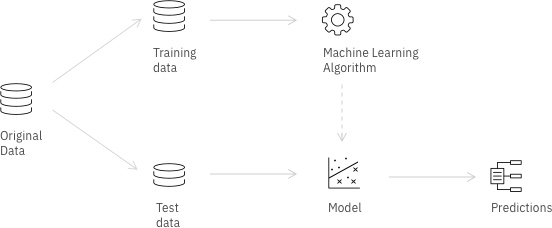
\includegraphics[scale=0.5]{images/ML_Process.jpg}
\caption {Processo padrão para aprendizado de máquina}
\label{fig:MLProcess}
\end{figure}

Um exemplo de arquitetura que generaliza todo o processo, desde a necessidade de negócio até o deploy do modelo de IA, é a IBM Analytics and AI Reference Architecture \citep{IBM_2021}, ilustrada na Figura \ref{fig:AIReferenceArchitecture}. Nela, são definidos os seguintes requisitos não-funcionais: Performance, estabilidade, segurança, escalabilidade, manutenibilidade e regulamentações de privacidade/\textit{compliance}, e pode ser classificada em 4 grupos principais envolvendo diversos tipos de processos e componentes:

\begin{figure}[h]
\centering
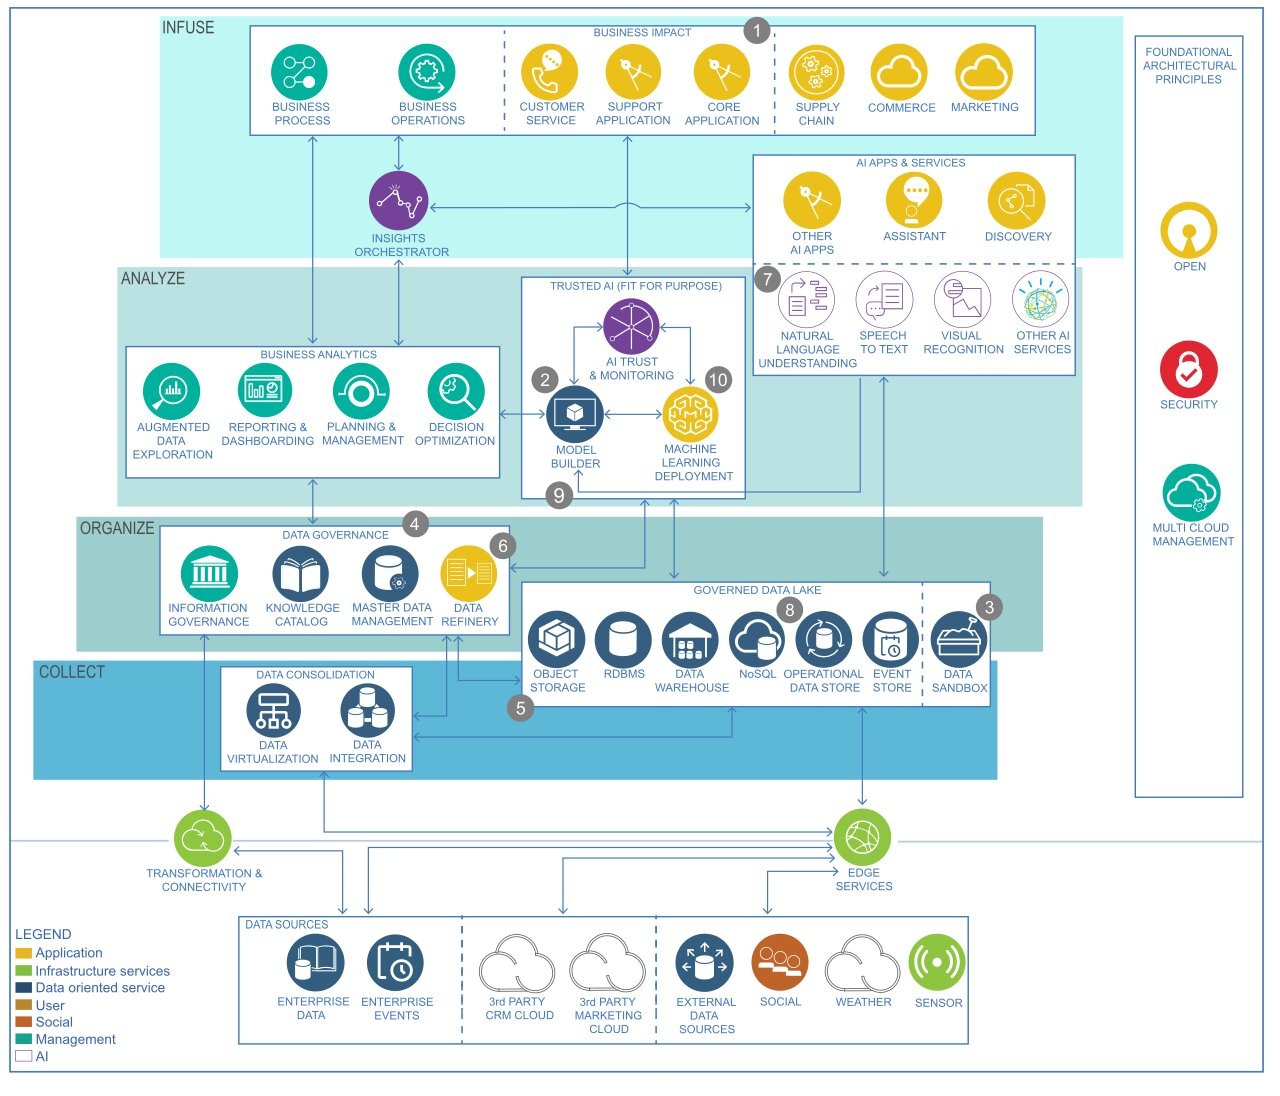
\includegraphics[scale=0.25]{images/ai-analytics-ref-diagram-analyze.jpg}
\caption {IBM Analytics and AI Reference Architecture.}
\label{fig:AIReferenceArchitecture}
\end{figure}

\begin{itemize}
\item \textbf{Coleta:} Relaciona os processos de coleta, armazenamento e transformação de diversas fontes de dados, estruturadas ou não estruturadas, para determinados repositórios (\textit{Data Lakes}).
\item \textbf{Organização:} Relaciona os processos de organização e estruturação dos dados nos presentes nos \textit{Data Lakes} e necessários para o uso das aplicações que envolvem a análise dos dados. Dependendo do uso pode-se aplicar processos de Governança.
\item \textbf{Análise:} Relaciona os processos para desenvolvimento de aplicações de IA e relatórios após a organização dos dados para tomadas de decisão e uso de aplicações externas.
\item \textbf{Infusão:} Relaciona os processos de disponibilização desses dados e conhecimento obtidos na fase de análise para aplicações externas.
\end{itemize}

\section{Proveniência de Dados}

\section{Arquitetura de Software}

O consenso sobre a definição de arquitetura de software foi adotado com a adoção do padrão IEEE 1471, que define arquitetura de software como \textit{"a organização fundamental de um sistema incorporado em seus componentes, seus relacionamentos entre si e com o meio ambiente e os princípios que orientam seu projeto e evolução"}. Com esta definição, o componente e o conector são reforçados como conceitos centrais da arquitetura de software~\citep{Bosch_2004}.

O nível de design da arquitetura de software em um projeto vai além dos algoritmos e estruturas de dados da computação. Incluem fatores como organização, protocolos de comunicação, acesso a dados, atribuição de funcionalidades, escalabilidade, performance, composição e seleção do \textit{design} ideal~\citep{Garlan_1993}. É possível tratar uma arquitetura de um sistema específico como uma coleção de componentes juntamente com uma descrição dos conectores, que define as interações entre os componentes.

Um estilo de arquitetura define uma família de tais sistemas em termos de um padrão de organização estrutural, e determina o vocabulário de componentes e conectores que podem ser usados em instâncias desse estilo, juntamente com um conjunto de restrições sobre como eles podem ser combinados~\citep{Garlan_1993}. A decisão sobre tal estilo depende da solução e dos requisitos de um sistema. Ela pode adicionar novos componentes, incrementá-los com novos requisitos ou adicionar restrições sobre eles~\citep{Bosch_2004}.

\subsection{Arquitetura MAPE-K}

Em 2001, Paul Horn introduziu o conceito de Computação Autônoma como alternativa a solução para a crescente complexidade dos sistemas da época, onde previa-se que os mesmos se tornariam muito grandes e complexos até mesmo para os profissionais mais qualificados configurarem e realizarem manutenção. Tal conceito qualifica sistemas de computação que podem se autogerenciar com relação aos objetivos de alto nível dados pelos administradores e é derivado da biologia, dado a grande variedade e hierarquia de sistemas autônomos presentes na natureza e na sociedade~\citep{Kephart_2003}. 

Em um ambiente autônomo e autogerenciado, os componentes de sistema podem incorporar como funcionalidade um \textit{loop} de controle. Embora estes \textit{loops} sejam divididos nos mesmos procedimentos, é possível categorizá-los em 4 categorias principais. Essas categorias são consideradas atributos dos componentes do sistema e são definidas como~\citep{IBM_2005}:

\begin{itemize}
\item \textbf{Auto-configuração:} Pode se adaptar dinamicamente a mudanças no ambiente. Um componente autoconfigurável realiza esta adaptação usando políticas fornecidas pelo profissional. Tais mudanças podem incluir a implantação de novos componentes ou a remoção dos existentes, ou mudanças drásticas nas características do sistema. A adaptação dinâmica ajuda a garantir força e produtividade contínuas da infraestrutura, resultando em crescimento e flexibilidade dos negócios.
\item \textbf{Auto-cura:} Pode descobrir, diagnosticar e reagir a interrupções. Um componente auto-curável pode detectar falhas no sistema e iniciar ações corretivas baseadas em políticas sem interromper o ambiente. A ação corretiva pode envolver um produto alterando seu próprio estado ou efetuando mudanças em outros componentes do ambiente. Com isso, o sistema se torna mais resiliente porque as operações cotidianas possuem menos probabilidade de falhar.
\item \textbf{Auto-otimização:} Pode monitorar e ajustar recursos automaticamente. Um componente auto-otimizável pode se ajustar para atender às necessidades do usuário. As ações de ajuste podem significar realocar recursos para melhorar a utilização geral, como em resposta a cargas de trabalho que mudam dinamicamente, ou garantir que processamentos possam ser concluídos em tempo hábil. A auto-otimização ajuda a fornecer um alto padrão de serviço para quem vai utilizar o sistema. Sem funções de auto-otimização, não há uma maneira fácil de re-escalonar os recursos de infraestrutura quando um aplicativo não os usa totalmente.
\item \textbf{Auto-proteção:} Pode antecipar, detectar, identificar e proteger contra ameaças de qualquer lugar. Um componente de autoproteção pode detectar comportamentos hostis à medida que ocorrem e tomar ações corretivas para se tornarem menos vulneráveis. Os comportamentos hostis podem incluir acesso e uso não autorizados, infecção e proliferação de vírus e ataques de negação de serviço. Os recursos de autoproteção permitem que as empresas apliquem consistentemente políticas de segurança e privacidade.
\end{itemize}

Para a Computação Autônoma acontecer, é implementado um Elemento Autônomo~\citep{Abbas_2010}, um componente de software que gerencia partes do sistema baseando-se em um \textit{loop} MAPE-K (\textit{Monitor, Analyze, Plan, Execute, and Knowledge}), ilustrado na Figura \ref{fig:MAPEK}. O MAPE-K é um conceito que constitui um \textit{loop} de controle, usado para monitorar e controlar um ou mais elementos gerenciados. Um elemento gerenciado (\textit{Managed Element}) pode ser um hardware, como uma impressora, um software, como um banco de dados, outro Elemento Autônomo ou funcões específicas, como balanceamento de carga. Um \textit{loop} de controle MAPE-K é dividido da seguinte forma:

\begin{itemize}
\item \textbf{Monitoramento (\textit{Monitor}):} Esta parte é responsável por monitorar os recursos gerenciados e coletar, agregar e filtrar dados. O monitoramento é feito por meio de um sensor (\textit{Sensor}) ou mais sensores.
\item \textbf{Análise (\textit{Analyze}):} Analisa os dados relatados pela parte do monitor. A análise visa compreender qual é o estado atual do sistema e se há medidas para serem tomadas.
\item \textbf{Planejamento (\textit{Plan}):} Um plano de ação é preparado no
base dos resultados da análise. O plano é uma série de medidas que irão mover o sistema de seu estado atual para um estado desejado.
\item \textbf{Execução (\textit{Execute}):} O plano é executado e controlado.
Um efetor (\textit{Effector}) ou mais executam as ações planejadas no recurso.
\item \textbf{Conhecimento (\textit{Knowledge}):} A base de conhecimento é central e acessível por todas as partes do \textit{loop}. Separado a partir de dados coletados e analisados, ele contém conhecimento adicional, como modelos de arquitetura, modelos de metas, políticas e planos de mudança.
\end{itemize}

\begin{figure}[h]
\centering
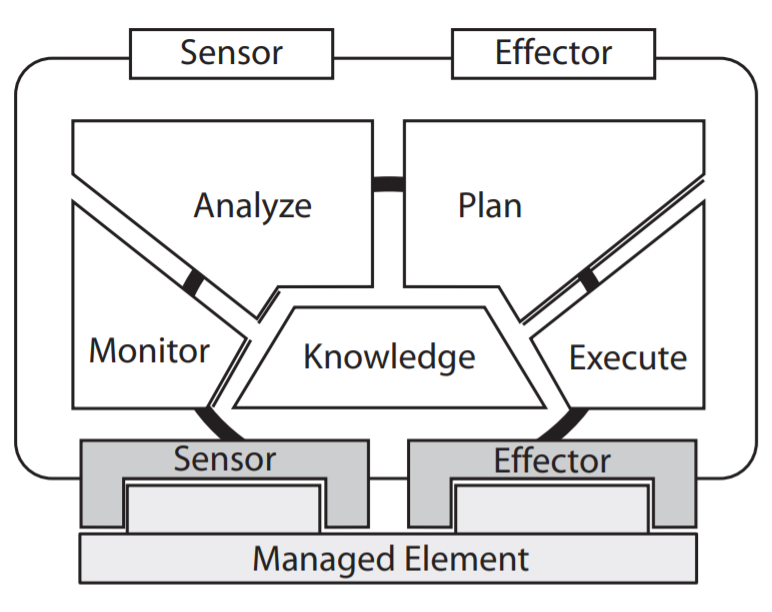
\includegraphics[scale=0.5]{images/MAPE-K.png}
\caption {Diagrama de funcionamento da arquitetura MAPE-K~\citep{Abbas_2010}.}
\label{fig:MAPEK}
\end{figure}

\subsection{Arquitetura \textit{Pipe-and-Filter}}

Em uma arquitetura \textit{Pipe-and-Filter}, ilustrado na Figura \ref{fig:PipeandFilter}, cada componente tem um conjunto de entradas e um conjunto de saídas. Um componente lê \textit{streams} (ou fluxos) de dados em suas entradas e produz \textit{streams} de dados em suas saídas, abstraindo a entrega de um resultado como um todo. O \textit{stream} de entrada é transformado de modo que a saída comece a ser produzida antes da entrada ser completamente consumida. Por isso, os componentes são chamados de filtros (\textit{filters}). Os conectores deste estilo servem como condutores para os \textit{streams}, transmitindo as saídas de um filtro para as entradas de outro. Por isso, os conectores são chamados de tubos (\textit{pipes})~\citep{Garlan_1993}.

\begin{figure}[h]
\centering
\includegraphics[scale=0.25]{images/PipeandFilter.png}
\caption {Diagrama de uma arquitetura \textit{Pipe-and-Filter}.}
\label{fig:PipeandFilter}
\end{figure}

Os filtros devem ser independentes, isto é, não devem compartilhar estado com outros filtros e, durante a programação, o ideal é que os filtros independam da ordem de processamento. Suas especificações podem restringir os dados transportados nos \textit{pipes} de entrada e nos \textit{pipes} de saída, mas não conhecem quaisquer outros filtros, ou componentes, conectados por seus \textit{pipes}. Especializações comuns desse estilo incluem \textit{pipelines}, que restringem as topologias a sequências lineares de filtros; \textit{Pipes} limitados, que restringem a quantidade de dados que podem ser passados em um \textit{pipe}, e \textit{pipes} tipados, que exigem que os dados passados entre dois filtros tenham um tipo bem definido.

O uso da arquitetura \textit{Pipe-and-Filter} possuí como vantagens:

\begin{itemize}
\item Permitem que o Arquiteto de Software/Desenvolvedor entendam o comportamento geral de entrada/saída de um sistema como uma composição simples dos comportamentos dos filtros individuais.
\item Suportam a reutilização: quaisquer dois filtros podem ser conectados, desde que concordem com os dados que estão sendo transmitidos entre eles. 
\item Os sistemas podem ser facilmente mantidos e aprimorados: novos filtros podem ser adicionados a sistemas existentes e filtros antigos podem ser substituídos por outros melhorados.
\item Permitem certos tipos de análise especializada, como análise de rendimento e de impasse.
\item Naturalmente suportam a execução simultânea: Cada filtro pode ser implementado como uma tarefa separada e potencialmente executado em paralelo com outros filtros.
\end{itemize}

Como desvantagens, é possível citar:

\begin{itemize}
\item Geralmente levam a uma organização de processamento em lote. Embora os filtros possam processar dados de forma incremental, uma vez que os filtros são inerentemente independentes, o Arquiteto de Software é forçado a pensar em cada filtro como fornecendo uma transformação completa dos dados de entrada em dados de saída. 
\item Por sua natureza de transformação de dados, os sistemas que usam a arquitetura \textit{Pipe-and-Filter} normalmente não são bons para lidar com aplicativos interativos. Esse problema é mais grave quando são necessárias atualizações de exibição incrementais, porque o padrão de saída para atualizações incrementais é radicalmente diferente do padrão para saída de filtro.
\item Podem ser prejudicados por terem que manter correspondências entre dois \textit{streams} separados, mas relacionados. 
\item Podem forçar um resultado médio na transmissão de dados em situações onde muitos filtros sejam encadeados com um único filtro, resultando em trabalho adicional para cada filtro separar seus dados e analisar o que for necessário. Isso, por sua vez, pode levar tanto à perda de desempenho quanto ao aumento da complexidade na escrita dos próprios filtros.
\end{itemize}

\chapter{Metodologia}
\label{sec:metodologia}

\section{Detalhamento do processo e diagramas elaborados}

\section{Arquitetura do código}

\section{Experimentos e limitações}

\chapter{Resultados e Discussões}

\chapter{Conclusões}



% As referências:
\bibliographystyle{plainnat}
\bibliography{full,thesis}

% Os anexos, se houver, vêm depois das referências:
%\backmatter
\appendix
\chapter{Conceitos complementares}

\section{AI Explainability}
\label{app:AIExplainability}

\textit{AI Explainability} é um conceito em IA que propõe a criação de um conjunto de técnicas de Aprendizado de Máquina (ou Machine Learning/ML) que produz modelos mais explicáveis, mantendo qualidade em suas métricas, e permite que os humanos entendam, confiem e gerenciem aplicações baseadas em IA. XAI também absorve conceitos das Ciências Sociais e considera a psicologia da explicação~\citep{Arrieta_2020}. Um algoritmo de ML explicável precisa não apenas mostrar tomadas de decisão, mas também mostrar o processo que o levou ao tomar tal decisão, de modo que seja compreensível e transparente para humanos.

\begin{figure}[h]
\centering
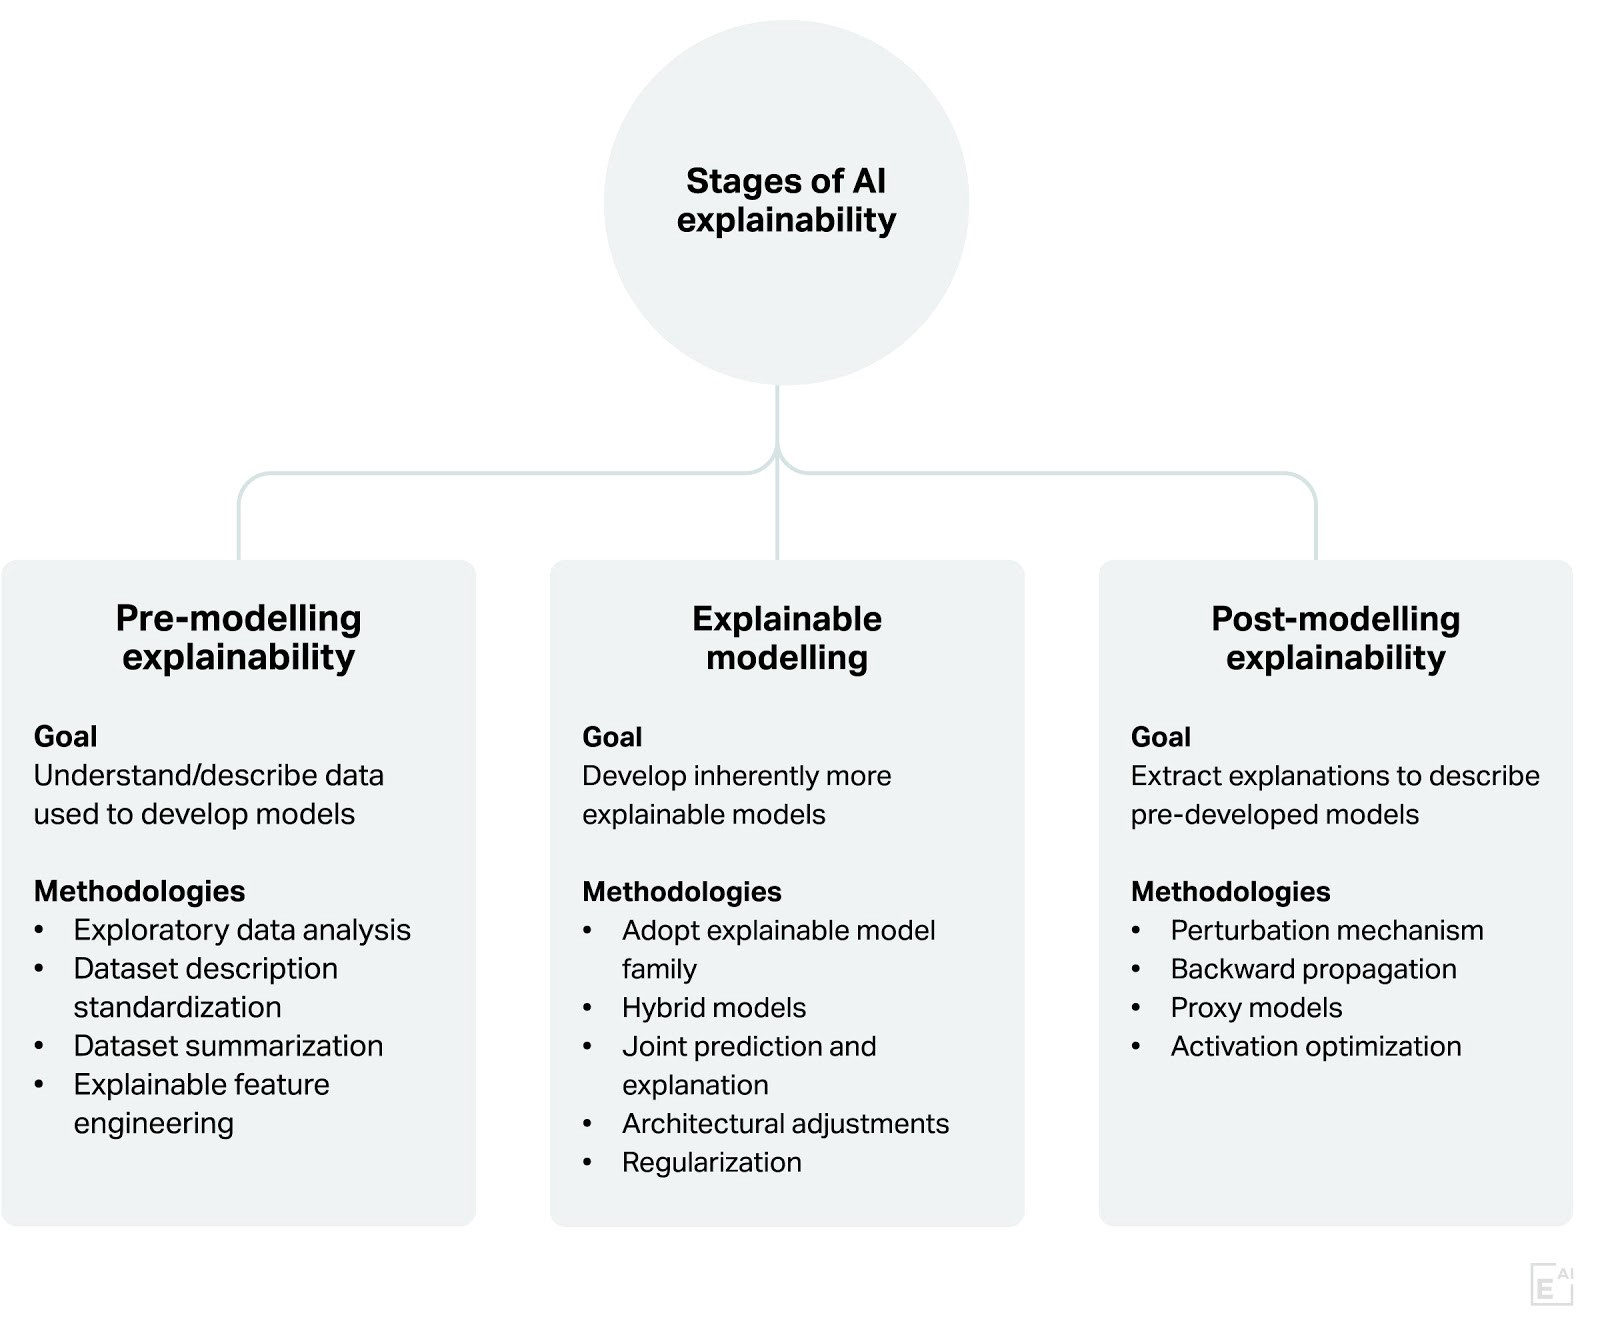
\includegraphics[scale=0.2]{images/phases.jpeg}
\caption {Fases de um processo baseado em IA explicável.}
\label{fig:StagesExplainableAI}
\end{figure}

Conforme ilustrado na Figura \ref{fig:StagesExplainableAI}, o um processo baseado em IA explicável pode ser classificado em 3 fases:

\begin{itemize}
\item \textbf{\textit{Pre-Modelling Explainability}:} Esta fase se caracteriza por obter explicações no conjunto de dados usado para treino e validação, tendo como principal motivação o fato do comportamento de um modelo depender muito dos dados que o alimentam. Análises e visualizações dos dados, ou mesmo através de documentações do conjunto de dados se enquadram neste estágio.~\citep{Khalegi_2019_Pre} 
\item \textbf{\textit{Explainable Modelling}:} Esta fase se caracteriza por obter explicações por modelos considerados transparentes (ver adiante). Ao adotar modelos deste tipo, ele já pode ser considerado como explicável por um humano. Também é possível obter a explicação através de regularizadores, ou adotar abordagens onde explicação e resultado sejam obtidos simultaneamente, sejam via junção de dados ou sendo intrínseco a arquitetura do modelo.~\citep{Khalegi_2019}
\item \textbf{\textit{Post-Modelling Explainability}:} Também chamada de \textit{Post-hoc Explainability} e onde a maioria dos trabalhos disponíveis baseados em XAI tenta focar, esta fase se dedica a explicar modelos desenvolvidos anteriormente, ou modelos que não são considerados como transparentes. Pode-se explicar um modelo por métodos como árvores de decisão e estimativas como valores de Shapley e propagação inversa.~\citep{Khalegi_2019_Post}
\end{itemize}

Entretanto, estas 3 fases não necessariamente são executadas de maneira sequencial: Por ser realizada no conjunto de dados e não no modelo, a fase de \textit{Pre-modelling Explainability} pode ser opcional, e a aplicação das fases de \textit{Explainable Modelling} e \textit{Post-Modelling Explainability} e seus métodos dependem exclusivamente se o modelo é classificado como transparente ou não, e tal critério é determinado pela adoção de uma (ou mais) das seguintes características~\citep{Arrieta_2020}:

\begin{itemize}
\item \textbf{Simulabilidade:} Denota a capacidade de um modelo de ser simulado ou pensado estritamente por um humano. A complexidade assume um lugar dominante nesta classe: Sistemas com uma grande quantidade de regras, por mais simples que essas sejam, já não podem ser classificados como tal. O modelo que se adequa a essa característica precisa ser autocontido o suficiente para que um ser humano pense e raciocine sobre ele como um todo.
\item \textbf{Decomponibilidade:} Também considerado como inteligibilidade, significa a capacidade de explicar cada uma das partes de um modelo. Se o modelo não for simples o suficiente, ele precisa ser divisível em várias pequenas partes e cada parte do modelo deve ser compreensível por um ser humano, sem a necessidade de ferramentas adicionais.
\item \textbf{Transparência do algoritmo:} Trata-se da habilidade do usuário de entender o processo seguido pelo modelo para produzir qualquer saída dada a partir de seus dados de entrada. Colocando de outra forma, um modelo linear é considerado transparente porque sua superfície de erro pode ser entendida e fundamentada, permitindo ao usuário entender como o modelo irá agir em cada situação que pode enfrentar.
\end{itemize}

\section{\textit{Fluent API}}
\label{app:FluentAPI}

O conceito de \textit{Fluent Interface}~\citep{Fowler_2005} (também conhecido como \textit{Fluent API}~\citep{Nakamaru_2020}) é uma abstração de código que o organiza de modo a criar uma \textit{Domain Specific Language} (DSL) interna, tendo como prioridade em seu \textit{design} a legibilidade e a fluidez. Embora a construção de uma \textit{Fluent API} consuma tempo, esse tempo pode ser recuperado com o tempo devido a maior facilidade no desenvolvimento e na manutenção dos componentes presentes no sistema.

Seu desenvolvimento lembra o \textit{Design Pattern} \textit{Builder}, onde seus métodos realizam acões específicas e retornam a referência do Objeto. Sua diferença está no objetivo em que foi desenvolvido: Enquanto no \textit{Builder} o objetivo está na construcão da instância de um Objeto, na \textit{Fluent API} o objetivo está em desenvolver uma série de ferramentas e ações de modo a resolver um problema específico.

A melhor forma de descrever e entender as diferenças e objetivos da Fluent API é através de um exemplo: O Código \ref{code:makeNormal} representa uma implementação padrão de um sistema, com instanciações de novos Objetos e métodos determinando atribuições e adição do elemento em uma lista.

\begin{lstlisting}[language=Java, label={code:makeNormal}, caption=Implementação padrão presente em um sistema~\citep{Fowler_2005}]
    private void makeNormal(Customer customer) {
        Order o1 = new Order();
        customer.addOrder(o1);
        OrderLine line1 = new OrderLine(6, Product.find("TAL"));
        o1.addLine(line1);
        OrderLine line2 = new OrderLine(5, Product.find("HPK"));
        o1.addLine(line2);
        OrderLine line3 = new OrderLine(3, Product.find("LGV"));
        o1.addLine(line3);
        line2.setSkippable(true);
        o1.setRush(true);
    }
\end{lstlisting}

O Código \ref{code:makeFluent} representa o mesmo sistema usando uma implementação com \textit{Fluent API}. Além na diminuição no número de linhas, a implementação é mais legível devido ao menor número de elementos presentes no código: Todas as chamadas e instanciações do Código \ref{code:makeNormal} estão ímplicitas, e o encadeamento das funções possui uma progressão lógica, mais sucinta e de simples entendimento.

\begin{lstlisting}[language=Java, label={code:makeFluent}, caption=Implementação com o uso de \textit{Fluent API}~\citep{Fowler_2005}]
   private void makeFluent(Customer customer) {
        customer.newOrder()
                .with(6, "TAL")
                .with(5, "HPK").skippable()
                .with(3, "LGV")
                .priorityRush();
    }
\end{lstlisting}

%\chapter{Apêndice}

%\annex
%\chapter{Anexo}
%\chapter{Anexo}


\end{document}
